Abbildung~\ref{fig:4_patterns} zeigt die Vorlagen für die 3 unterschiedlichen Zeichen \texttt{8}, \texttt{3} und \texttt{0}. Aus diesen Patterns wurde durch Addieren mit zufälligen Werten ein Satz von Trainingsdaten generiert, mit dem ein neuronales Netzwerk mit 2 Hidden Neuronen trainiert wurde. Dabei wurde eine Klassifizierungsgenauigkeit von 100\% erreicht.

\begin{figure}[h!]
  \begin{center}
    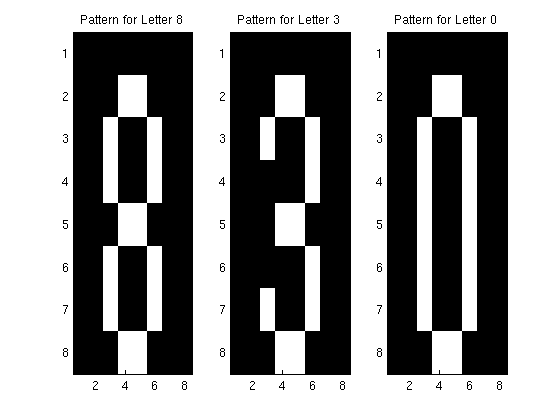
\includegraphics[width=0.75\textwidth]{./figures/4_patterns}
    \caption{Patterns für die unterschiedlichen Zeichen}
    \label{fig:4_patterns}
  \end{center}
\end{figure}

Abbildung~\ref{fig:4_weights} zeigt die Gewichte zwischen Input und Hidden Neuronen. 

\begin{figure}[h!]
  \begin{center}
    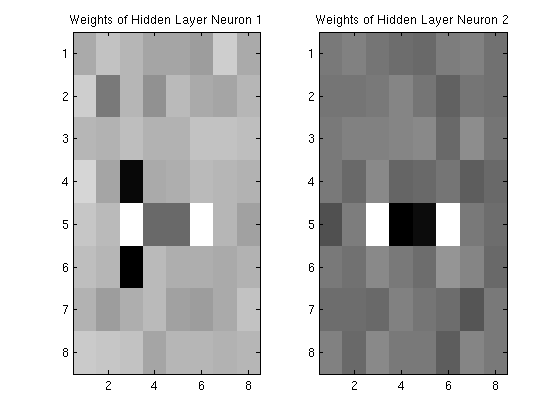
\includegraphics[width=0.75\textwidth]{./figures/4_weights}
    \caption{Gewichte zwischen Input und Hidden Neuronen}
    \label{fig:4_weights}
  \end{center}
\end{figure}

Man erkennt, dass die Gewichte die Bereiche in den Patterns hervorheben, die zum Unterscheiden der Patterns wichtig sind (\emph{Features}). Diese Bereiche haben in den Gewichtsmatrizen den gleichen Wert. Vergleicht man Abbildungen \ref{fig:4_patterns} und \ref{fig:4_weight}, fällt sofort auf, dass die Bereiche, die in den Patterns unterschiedlich sind (und damit die wichtigsten Merkmale) in den Gewichtsmatrizen besonders herausstechen. Dabei haben die Elemente, bei denen sich die Patterns \texttt{8} und \texttt{3} unterscheiden einen anderen Wert als z.B. die Elemente, bei denen sich die Patterns \texttt{8} und \texttt{0} unterscheiden. Dadurch kann das neuronale Netzwerk durch richtiges gewichtetes Addieren (Hidden Layer $\rightarrow$ Output Layer) Ausgänge erzeugen, von denen bei richtig erkannten Zeichen jeweils nur einer aktiv wird, sprich Output-Neuron \texttt{0} reagiert z.B. auf einen hohen Wert von Hidden-Neuron 1 \emph{und} einen hohen Wert von Hidden-Neuron 2. Das passiert, wenn die Elemente, bei denen die Gewichte hoch sind (in Abb.~\ref{fig:4_weights} weiß) ebenfalls hoch sind (in Abb.~\ref{fig:4_patterns}), was für Daten, die das Zeichen \texttt{0} repräsentieren zutrifft.

